\chapter{LapOps}


\section{Introduction}

\section{Core idea of the project}
The idea behind the project was to create an application that records a driven lap with a car or a go-kart and returns a result, that identifies the fastest lap and compares to other laps to that. Our core problem, that we identified in our project is the identification of the track sections. After discussion, we reached a consensus, that our application should be able to identify curves and straights reliable. The first sketch is visible in figure \ref{sketchLapOps} which shows the idea of splitting a track into sections. The last step would be to compare the same sections in different laps to get improvement tips.

\begin{figure}[H]
	\centering
	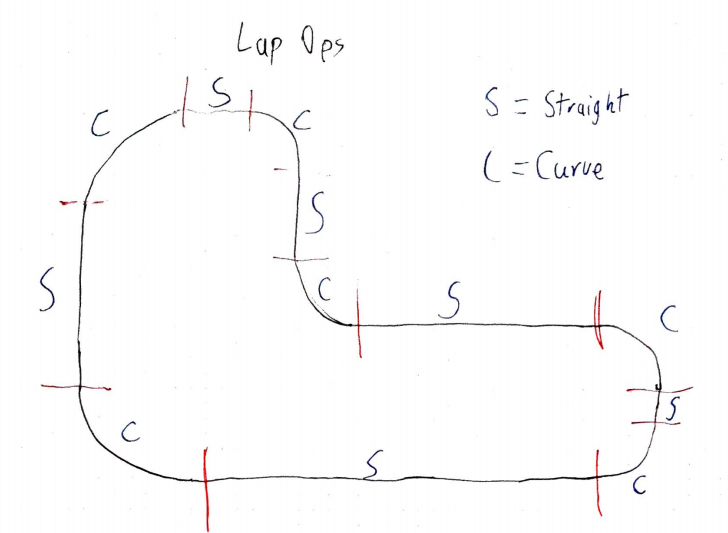
\includegraphics[scale= 0.6]{Pictures/LapOpsSkizze.png}
	\caption{Sketch of the core idea of section identification}
	\label{sketchLapOps}
\end{figure}
